%%%%%%%%%%%%%%%%%%%%%%%%%%%%%%%%%%%%%%%%%%%%%%%%%%%%%%%%%%%%%%%%%%%%%%%%%%%%%%%%
%%%%%%%%%%%%%%%%%%%%%%%%%%%%%%%%%%%%%%%%%%%%%%%%%%%%%%%%%%%%%%%%%%%%%%%%%%%%%%%%
%%%%%%%%%%%%%%%%%%%%%%%%%%%%%%%%%%%%%%%%%%%%%%%%%%%%%%%%%%%%%%%%%%%%%%%%%%%%%%%%
%%%%%%%%%%%%%%%%%%%%%%%%%%%%%%%%%%%%%%%%%%%%%%%%%%%%%%%%%%%%%%%%%%%%%%%%%%%%%%%%
\chapter{Transformée de Laplace inverse~\label{annexe-invL}}
%%%%%%%%%%%%%%%%%%%%%%%%%%%%%%%%%%%%%%%%%%%%%%%%%%%%%%%%%%%%%%%%%%%%%%%%%%%%%%%%
%%%%%%%%%%%%%%%%%%%%%%%%%%%%%%%%%%%%%%%%%%%%%%%%%%%%%%%%%%%%%%%%%%%%%%%%%%%%%%%%
%%%%%%%%%%%%%%%%%%%%%%%%%%%%%%%%%%%%%%%%%%%%%%%%%%%%%%%%%%%%%%%%%%%%%%%%%%%%%%%%
%%%%%%%%%%%%%%%%%%%%%%%%%%%%%%%%%%%%%%%%%%%%%%%%%%%%%%%%%%%%%%%%%%%%%%%%%%%%%%%%

%%%%%%%%%%%%%%%%%%%%%%%%%%%%%%%%%%%%%%%%%%%%%%%%%%%%%%%%%%%%%%%%%%%%%%%%%%%%%%%%
%%%%%%%%%%%%%%%%%%%%%%%%%%%%%%%%%%%%%%%%%%%%%%%%%%%%%%%%%%%%%%%%%%%%%%%%%%%%%%%%
%%%%%%%%%%%%%%%%%%%%%%%%%%%%%%%%%%%%%%%%%%%%%%%%%%%%%%%%%%%%%%%%%%%%%%%%%%%%%%%%
\section{Contexte}
%%%%%%%%%%%%%%%%%%%%%%%%%%%%%%%%%%%%%%%%%%%%%%%%%%%%%%%%%%%%%%%%%%%%%%%%%%%%%%%%
%%%%%%%%%%%%%%%%%%%%%%%%%%%%%%%%%%%%%%%%%%%%%%%%%%%%%%%%%%%%%%%%%%%%%%%%%%%%%%%%
%%%%%%%%%%%%%%%%%%%%%%%%%%%%%%%%%%%%%%%%%%%%%%%%%%%%%%%%%%%%%%%%%%%%%%%%%%%%%%%%
Il existe une forme analytique de la transformée inverse basée sur
la formule de Mellin-Fourier\cite{Ostertag}:
\[
s(t)=\laplacei{S(p)}=\int_{c-j\infty}^{c+j\infty} e^{pt}S(p)\dd{p}
\]
Cette inversion se fait donc par le biais d'une intégrale dans le plan
complexe. Cette intégrale n'ayant pas de forme analytique, il n'est possible 
d'approcher une solution qu'à l'aide d'outils numérique. 
Dans cette annnexe, nous discuterons deux implémentations en python de 
deux de ces algorithmes : 
l'algorithme de Gaver-Stehfest et l'algorithme fixe de Talbot comme présentés
par Abate et al.~\cite{abate2004,abate2006,frwiki:200676411}.
Avant de tester ces méthodes sur les systèmes linéaires, nous l'appliquerons
à l'inversion de Laplace :  
\[
    te^{-t}=\laplacei{\dfrac{1}{(p+1)^2}},
\]
dont on connait la forme analytique exacte.
%%%%%%%%%%%%%%%%%%%%%%%%%%%%%%%%%%%%%%%%%%%%%%%%%%%%%%%%%%%%%%%%%%%%%%%%%%%%%%%%
%%%%%%%%%%%%%%%%%%%%%%%%%%%%%%%%%%%%%%%%%%%%%%%%%%%%%%%%%%%%%%%%%%%%%%%%%%%%%%%%
%%%%%%%%%%%%%%%%%%%%%%%%%%%%%%%%%%%%%%%%%%%%%%%%%%%%%%%%%%%%%%%%%%%%%%%%%%%%%%%%
\section{Algorithme de Gaver-Stehfest}
%%%%%%%%%%%%%%%%%%%%%%%%%%%%%%%%%%%%%%%%%%%%%%%%%%%%%%%%%%%%%%%%%%%%%%%%%%%%%%%%
%%%%%%%%%%%%%%%%%%%%%%%%%%%%%%%%%%%%%%%%%%%%%%%%%%%%%%%%%%%%%%%%%%%%%%%%%%%%%%%%
%%%%%%%%%%%%%%%%%%%%%%%%%%%%%%%%%%%%%%%%%%%%%%%%%%%%%%%%%%%%%%%%%%%%%%%%%%%%%%%%
La transformée inverse par la méthode de Gaver-Stehfest est donné par 
(relation adaptée de l'équation (31) de~\cite{abate2006}) :
\[
f(t)=\dfrac{\ln{2}}{t}\sum_{k=1}^{2M}\zeta_kF\left(\dfrac{k\ln{2}}{t}\right)
\]
où l'on note $f(t)$ la fonction inverse de $F(p)$ et les $\zeta_k$ sont
donnés par la relation (32) de~\cite{abate2006} c'est à dire :
\[
\zeta_k = (-1)^{M+k} \sum_{j=\lfloor(k+1)/2\rfloor}^{\min{(k,M)}} 
\dfrac{j^{M+1}}{M!}\begin{pmatrix} M\\j  \end{pmatrix}
                   \begin{pmatrix} 2j\\j \end{pmatrix}
                   \begin{pmatrix} j\\k-j\end{pmatrix}
\]
avec $\lfloor x \rfloor$ le plus grand entier inférieur ou égal à $x$. Il 
nous faudra définir les coefficients binomiaux et les $\zeta_k$ avec les
deux fonctions suivantes :
\clearpage
%-------------------------------------------------------------------------------
\inputminted{python}{codes/python/coeff_bin-annexe_invL.py}
%-------------------------------------------------------------------------------
%-------------------------------------------------------------------------------
\inputminted{python}{codes/python/zeta-annexe_invL.py}
%-------------------------------------------------------------------------------
La fonction \texttt{gaver\_stehfest} qui prend en paramètres 
le temps \texttt{t} et la fonction \texttt{f} représentant la fonction $f(t)$ 
inverse de $F(p)$.
%-------------------------------------------------------------------------------
\inputminted{python}{codes/python/gaver_stehfest-annexe_invL.py}
%-------------------------------------------------------------------------------
%%%%%%%%%%%%%%%%%%%%%%%%%%%%%%%%%%%%%%%%%%%%%%%%%%%%%%%%%%%%%%%%%%%%%%%%%%%%%%%%
%%%%%%%%%%%%%%%%%%%%%%%%%%%%%%%%%%%%%%%%%%%%%%%%%%%%%%%%%%%%%%%%%%%%%%%%%%%%%%%%
\subsection*{Test de la méthode}
%%%%%%%%%%%%%%%%%%%%%%%%%%%%%%%%%%%%%%%%%%%%%%%%%%%%%%%%%%%%%%%%%%%%%%%%%%%%%%%%
%%%%%%%%%%%%%%%%%%%%%%%%%%%%%%%%%%%%%%%%%%%%%%%%%%%%%%%%%%%%%%%%%%%%%%%%%%%%%%%%
Soit la transformée de Laplace inverse connue :
\[
    te^{-t}=\laplacei{\dfrac{1}{(p+1)^2}}
\]
Que l'on écrit sous forme de fonctions de la façon suivante en python:
\begin{minted}{python}
ft=lambda t : t*m.exp(-t)
fp=lambda p : 1/(p+1)**2
\end{minted}
On cherche à déterminer la transformée inverse pour différentes valeurs
de $t\in[10^{-4},10^4]$  
\begin{minted}{python}
t=np.logspace(-4,4,256)
f_gaver_stehfest=np.array([gaver_stehfest(tk,fp,20) for tk in t])
f_analytic=np.array([ft(tk) for tk in t])
\end{minted}
Nous traçons ci-dessous la différence relative :
\[
    f_{\textrm{stehfest}}(t) - f_{\textrm{exact}}(t) 
\]

%-------------------------------------------------------------------------------
\begin{figure}[!b]
    \centering
    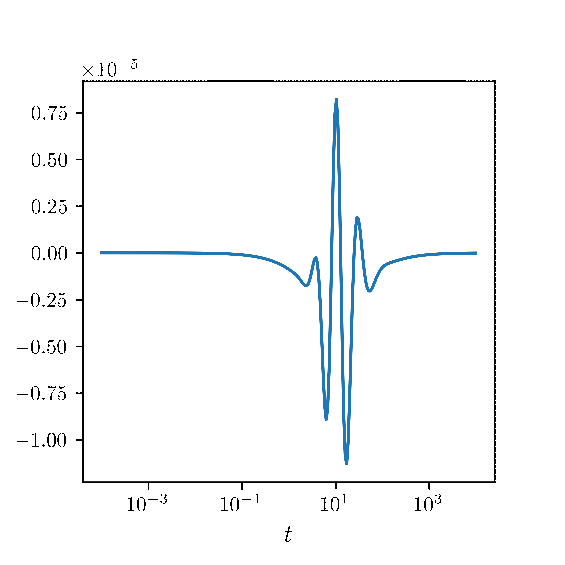
\includegraphics[width=0.65\linewidth]{erreur_gaver-stehfest.eps}
    \caption{Erreur relative entre l'approche de Gaver-Stehfest et 
             la relation exacte}
\end{figure}
%-------------------------------------------------------------------------------
\clearpage
%%%%%%%%%%%%%%%%%%%%%%%%%%%%%%%%%%%%%%%%%%%%%%%%%%%%%%%%%%%%%%%%%%%%%%%%%%%%%%%%
%%%%%%%%%%%%%%%%%%%%%%%%%%%%%%%%%%%%%%%%%%%%%%%%%%%%%%%%%%%%%%%%%%%%%%%%%%%%%%%%
%%%%%%%%%%%%%%%%%%%%%%%%%%%%%%%%%%%%%%%%%%%%%%%%%%%%%%%%%%%%%%%%%%%%%%%%%%%%%%%%
\section{Algorithme fixe de Talbot}
%%%%%%%%%%%%%%%%%%%%%%%%%%%%%%%%%%%%%%%%%%%%%%%%%%%%%%%%%%%%%%%%%%%%%%%%%%%%%%%%
%%%%%%%%%%%%%%%%%%%%%%%%%%%%%%%%%%%%%%%%%%%%%%%%%%%%%%%%%%%%%%%%%%%%%%%%%%%%%%%%
%%%%%%%%%%%%%%%%%%%%%%%%%%%%%%%%%%%%%%%%%%%%%%%%%%%%%%%%%%%%%%%%%%%%%%%%%%%%%%%%
On souhaite se donner la relation (18) de~\cite{abate2004} 
qui se présente sous la forme :
\[
f(t) = \dfrac{r}{M} 
\left\{ 
    \dfrac{1}{2} F(r) e^{rt}+ \sum_{k=1}^{M-1} 
    \textrm{Re}\left[ e^{ts(\theta_k)} F(s(\theta_k)) (1+i\sigma(\theta_k))\right]
\right\}
\]
avec $\theta_k=\frac{k\pi}{M}$, et les relations (19), (16) et (11) de [3] 
sont nécessaires pour implémenter la méthode à savoir 
$r=\frac{2M}{5t}$,$\sigma(\theta)=\theta+(\theta\cot\theta-1)\cot\theta$,
$s(\theta)=r\theta(\cot\theta+i)$.
\inputminted{python}{codes/python/talbot-annexe_invL.py}
%%%%%%%%%%%%%%%%%%%%%%%%%%%%%%%%%%%%%%%%%%%%%%%%%%%%%%%%%%%%%%%%%%%%%%%%%%%%%%%%
%%%%%%%%%%%%%%%%%%%%%%%%%%%%%%%%%%%%%%%%%%%%%%%%%%%%%%%%%%%%%%%%%%%%%%%%%%%%%%%%
\subsection*{Test de la méthode}
%%%%%%%%%%%%%%%%%%%%%%%%%%%%%%%%%%%%%%%%%%%%%%%%%%%%%%%%%%%%%%%%%%%%%%%%%%%%%%%%
%%%%%%%%%%%%%%%%%%%%%%%%%%%%%%%%%%%%%%%%%%%%%%%%%%%%%%%%%%%%%%%%%%%%%%%%%%%%%%%%
Nous cherchons à nouveau à reproduire la transformée de Laplace inverse connue :
\[
    te^{-t}=\laplacei{\dfrac{1}{(p+1)^2}}
\]
Nous traçons ci-dessous la différence relative pour différence valeurs de $t$:
\[
    f_{\textrm{talbot}}(t) - f_{\textrm{exact}}(t) 
\]
%-------------------------------------------------------------------------------
\begin{figure}[!b]
    \centering
    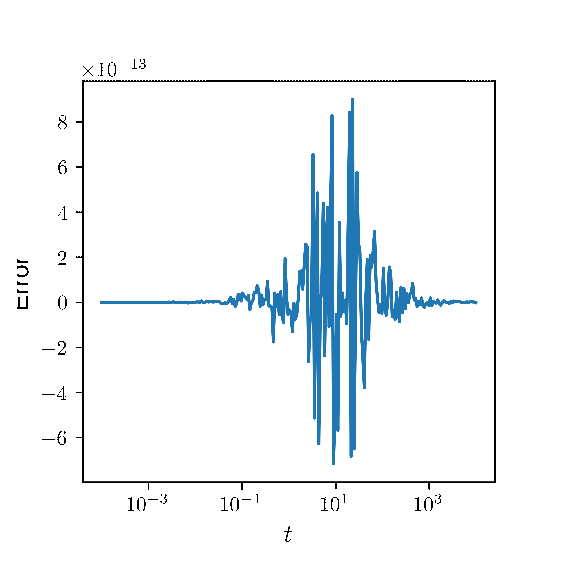
\includegraphics[width=0.65\linewidth]{erreur_talbot.eps}
    \caption{Erreur relative entre l'algorithme fixe de Talbot et 
             la relation exacte.}
\end{figure}
%-------------------------------------------------------------------------------
\clearpage
%%%%%%%%%%%%%%%%%%%%%%%%%%%%%%%%%%%%%%%%%%%%%%%%%%%%%%%%%%%%%%%%%%%%%%%%%%%%%%%%
%%%%%%%%%%%%%%%%%%%%%%%%%%%%%%%%%%%%%%%%%%%%%%%%%%%%%%%%%%%%%%%%%%%%%%%%%%%%%%%%
%%%%%%%%%%%%%%%%%%%%%%%%%%%%%%%%%%%%%%%%%%%%%%%%%%%%%%%%%%%%%%%%%%%%%%%%%%%%%%%%
\section{Exemple d'applications aux SLCI}
%%%%%%%%%%%%%%%%%%%%%%%%%%%%%%%%%%%%%%%%%%%%%%%%%%%%%%%%%%%%%%%%%%%%%%%%%%%%%%%%
%%%%%%%%%%%%%%%%%%%%%%%%%%%%%%%%%%%%%%%%%%%%%%%%%%%%%%%%%%%%%%%%%%%%%%%%%%%%%%%%
%%%%%%%%%%%%%%%%%%%%%%%%%%%%%%%%%%%%%%%%%%%%%%%%%%%%%%%%%%%%%%%%%%%%%%%%%%%%%%%%

\inputminted{python}{codes/python/1er_ordre-annexe_invL.py}
\inputminted{python}{codes/python/2nd_ordre-annexe_invL.py}

%1er_ordre_talbot.eps  2nd_ordre_talbot.eps  erreur_gaver-stehfest.eps  erreur_talbot.eps
\begin{figure}
    \centering
    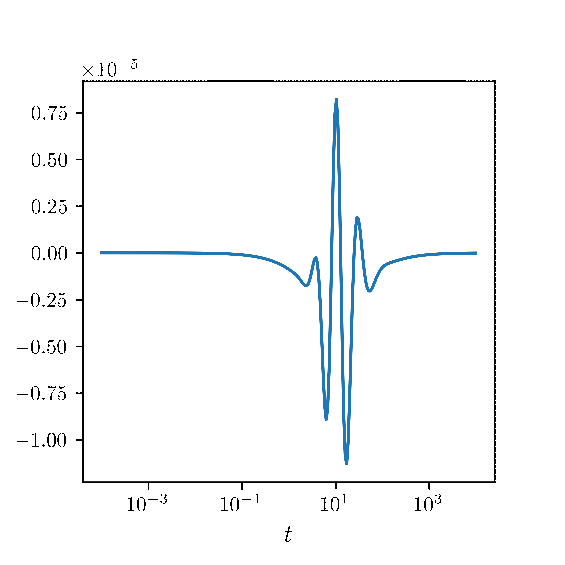
\includegraphics[width=0.8\linewidth]{erreur_gaver-stehfest.eps}
\end{figure}
%%%%%%%%%%%%%%%%%%%%%%%%%%%%%%%%%%%%%%%%%%%%%%%%%%%%%%%%%%%%%%%%%%%%%%%%%%%%%%%%
%%%%%%%%%%%%%%%%%%%%%%%%%%%%%%%%%%%%%%%%%%%%%%%%%%%%%%%%%%%%%%%%%%%%%%%%%%%%%%%%
%%%%%%%%%%%%%%%%%%%%%%%%%%%%%%%%%%%%%%%%%%%%%%%%%%%%%%%%%%%%%%%%%%%%%%%%%%%%%%%%
%%%%%%%%%%%%%%%%%%%%%%%%%%%%%%%%%%%%%%%%%%%%%%%%%%%%%%%%%%%%%%%%%%%%%%%%%%%%%%%%
%annexe_invL.tex
